\newpage
\paragraph{LDM}\mbox{}\\

In this attempt $z$ was sampled from $\mathcal{N}(0,1)$ and passed through the latent diffusion model, which was the denoising U-Net from the Monai framework. 

\subparagraph{Configuration}\mbox{}\\

\begin{table}[H]
\centering
\begin{tabular}{|l|l|}
\hline
\textbf{Parameter} & \textbf{Value} \\
\hline
\multicolumn{2}{|c|}{\textbf{Training}} \\
\hline
Batch Size & 5 \\
\hline
Seed & 42 \\
\hline
Epochs & 15000 \\
\hline
Training Ratio & 0.9 \\
\hline
Number of Nodes & 1 \\
\hline
Device & CUDA \\
\hline
\multicolumn{2}{|c|}{\textbf{Model}} \\
\hline
Spatial Dimensions & 3 \\
\hline
Input Channels & 3 \\
\hline
Output Channels & 3 \\
\hline
Number of Residual Blocks & 1 \\
\hline
Number of Channels & [32, 64, 64] \\
\hline
Attention Levels & [False, True, True] \\
\hline
Number of Head Channels & [0, 64, 64] \\
\hline
Number of Training Steps & 1000 \\
\hline
Beta Start & 0.0015 \\
\hline
Beta End & 0.0195 \\
\hline
Schedule & Scaled Linear Beta \\
\hline
Learning Rate & 0.0002 \\
\hline
Scale Factor & 1.0049688816070557 \\
\hline
Autoencoder Checkpoint Path & \url{./models/monai_autoencoder/}\\ 
& \url{checkpoints/monai_autoencoder-v5.ckpt} \\
\hline
Scan Shape & [1, 128, 128, 32] \\
\hline
Beta1 & 0.5 \\
\hline
Beta2 & 0.999 \\
\hline
\multicolumn{2}{|c|}{\textbf{Dataset}} \\
\hline
Caching & Disk \\
\hline
Path & \url{/ravana/d3d\_work/micorl/data/ct\_images\_prostate\_32fixed/} \\
\hline
Image Size & 128 \\
\hline
Number of Slices & 32 \\
\hline
Window Width & 400 \\
\hline
Window Level & 60 \\
\hline
\end{tabular}
\caption{Configuration of the MONAI Diffuser.}
\label{table:monai_diffuser_params}
\end{table}

\newpage
\subparagraph{Training}\mbox{}\\

The model was trained for 15000 epochs. Training loss decreased to a low level before even 1000 epoch was reached. However, the validation loss continued to vary around 1 (Fig. \ref{fig:ldm_a1_val_loss}). 

\begin{figure}[H]
\minipage{0.49\textwidth}
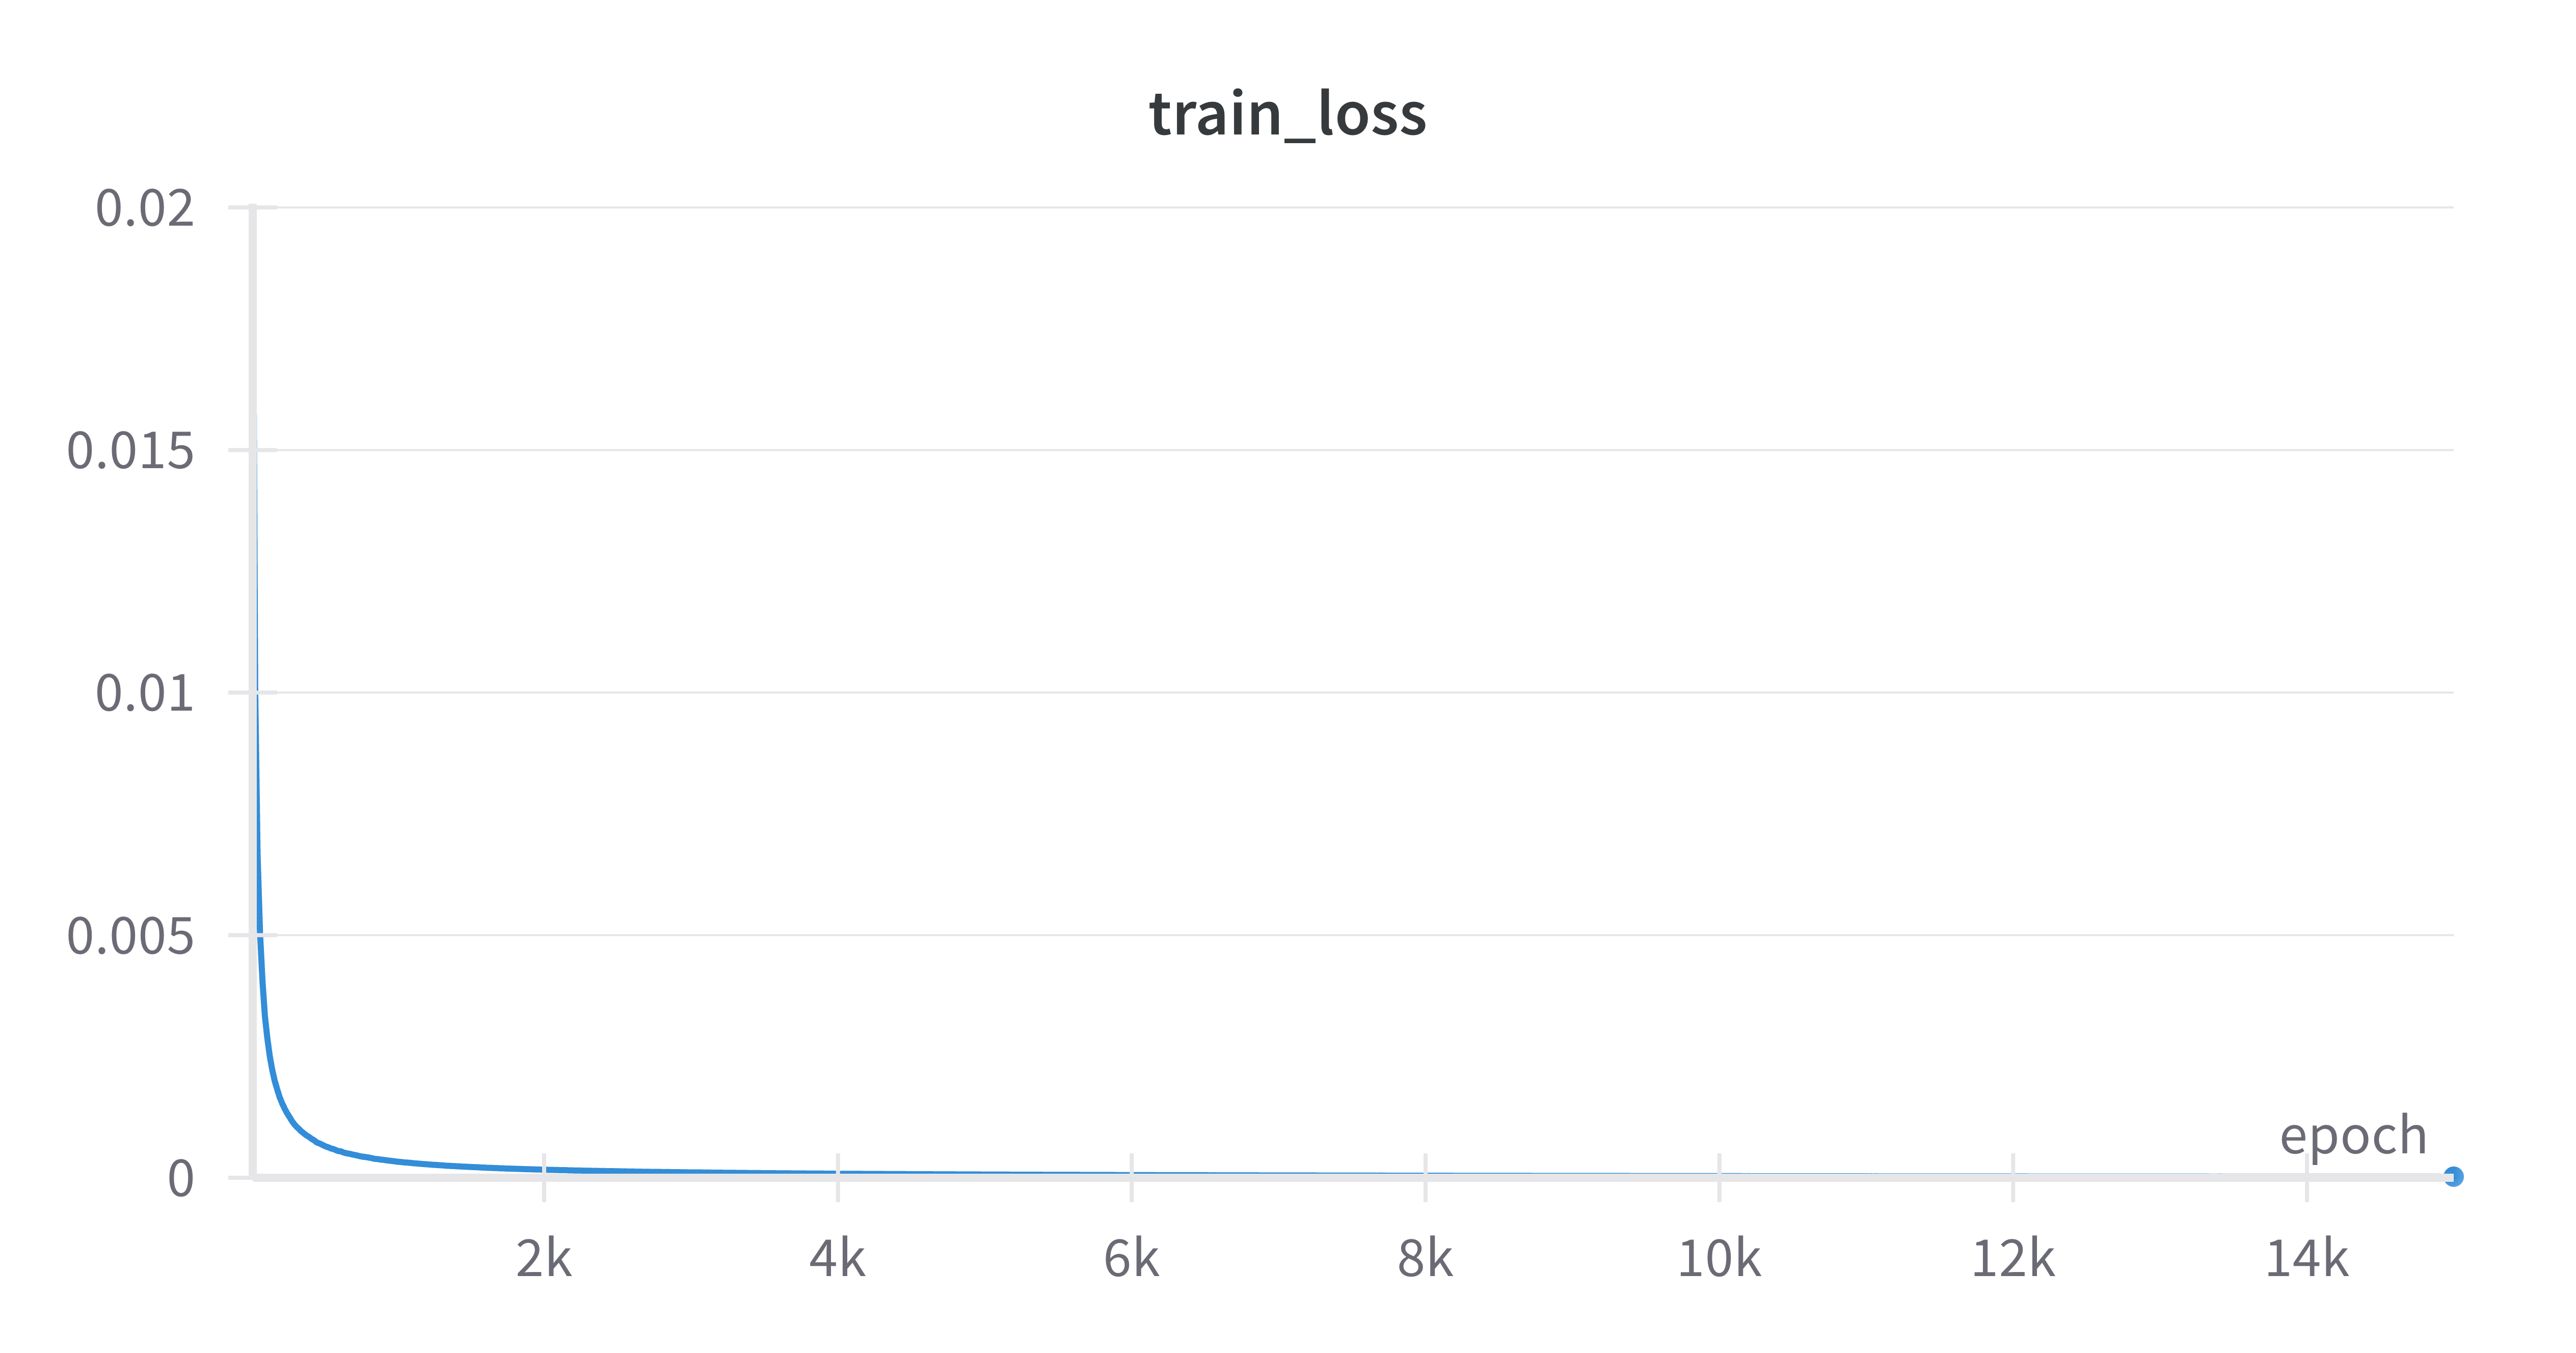
\includegraphics[width=\linewidth]{detailed_engineering/Monai Diffusion - Attempt 1/charts/train_loss.png}
\caption{Loss during the training.}
\endminipage\hfill
\minipage{0.49\textwidth}
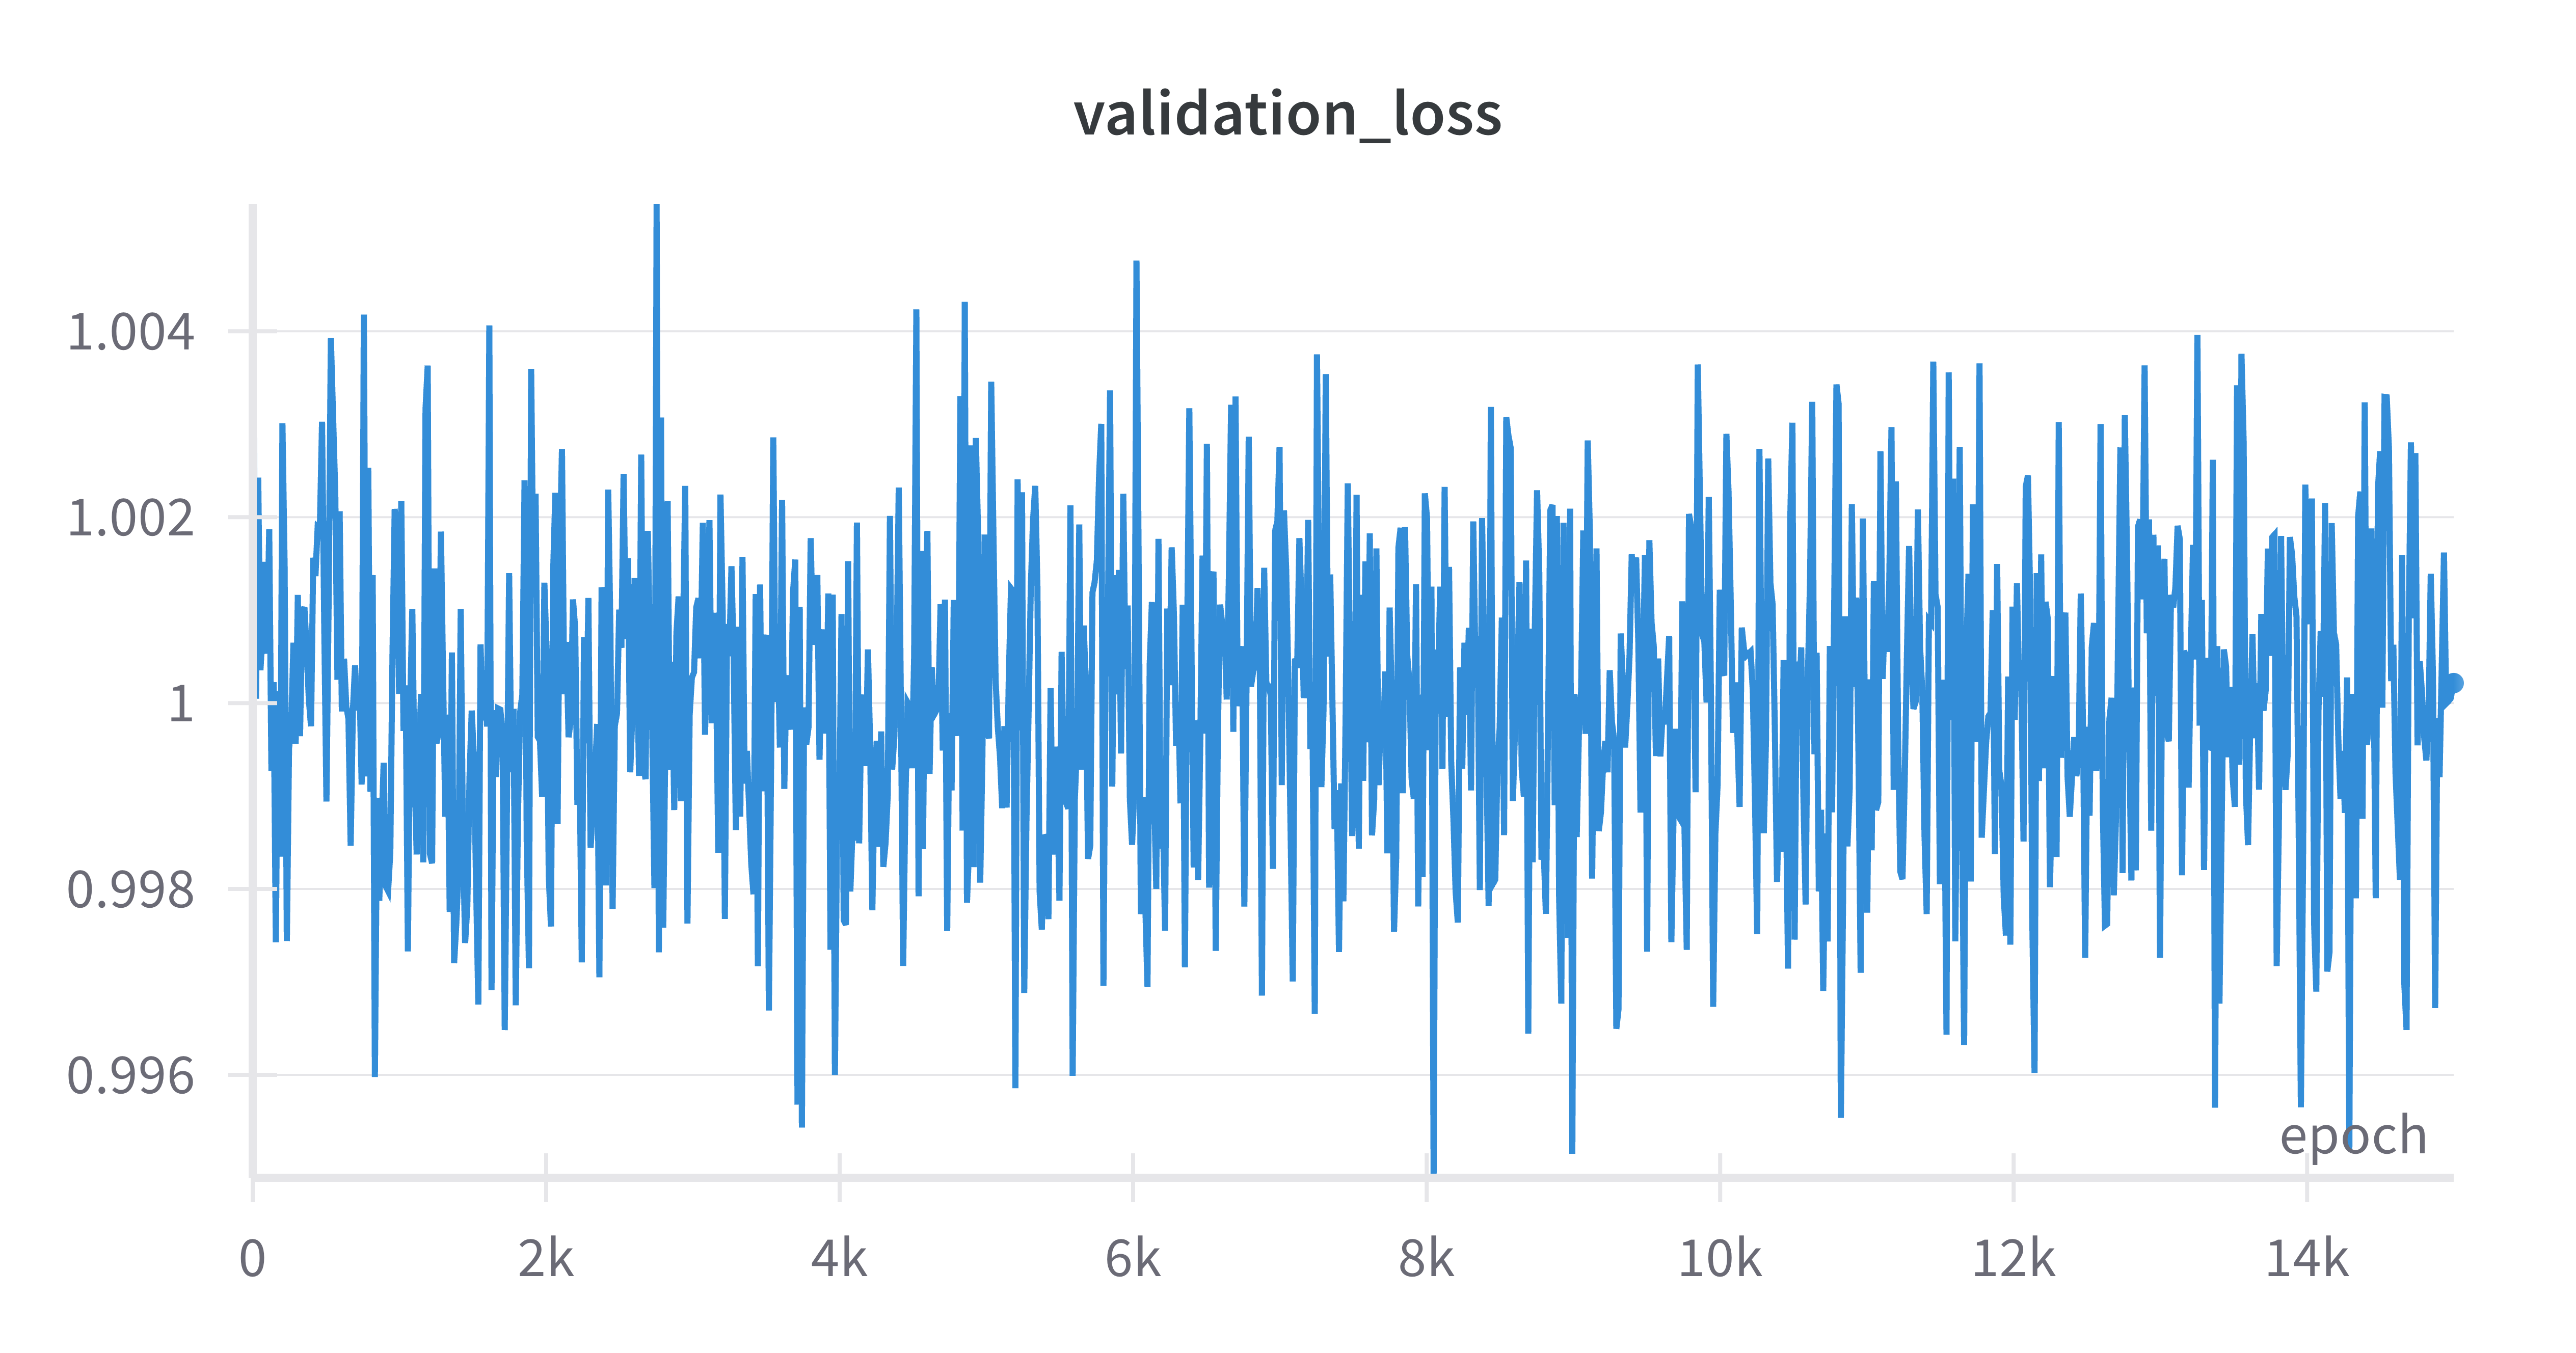
\includegraphics[width=\linewidth]{detailed_engineering/Monai Diffusion - Attempt 1/charts/validation_loss.png}
\caption{Loss during the validation.}
\label{fig:ldm_a1_val_loss}
\endminipage
\end{figure}


\subparagraph{Results}\mbox{}\\

\begin{figure}[H]
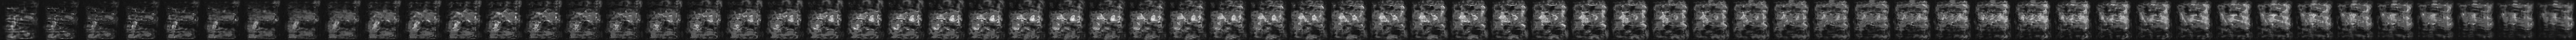
\includegraphics[width=\linewidth]{detailed_engineering/Monai Diffusion - Attempt 1/charts/generation.png}
\caption{Unsuccessful generation of a synthetic CT scan.}
\label{fig:attempt1-generation}
\end{figure}

\indent Generation was unsuccessful as shown in Figure \ref{fig:attempt1-generation}. The resulting image looks like structured noise instead of a CT scan. The validation loss did not decrease (Fig. \ref{fig:ldm_a1_val_loss}). It seems like a prior collapse occurred and the decoder did not perceive generated latent representation as useful information during the decoding.
